La natura delle informazioni in possesso si riflette sulla tipologia dei modelli di machine learning utilizzabili. Oltre alla diversificazione in strutturati e non-strutturati, i dati possono essere ulteriormente contraddistinti in \textbf{etichettati} e \textbf{non-etichettati}. Si osservino i titoli esemplificativi riportati di seguito, pur di comprendere la sottile differenza che li distingue. Entrambi i formati tabellari raffigurano dei dataset relativi a fenomeni celesti.
\begin{figure}[H]
    \centering
    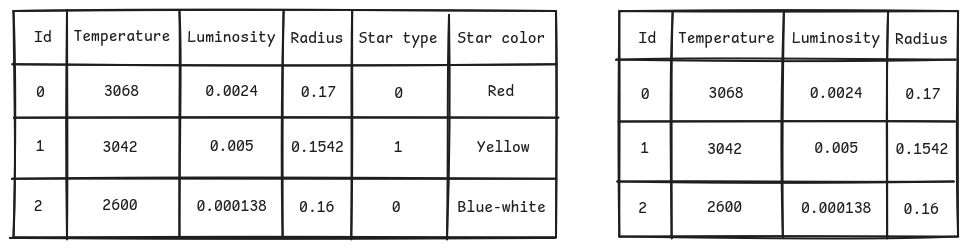
\includegraphics[width=1.0\linewidth]{img/img1.png}
    \caption{Contrapposizione tra dataset con dati etichettati e non-etichettati}
\end{figure}
Come da immagine, la prima tabella possiede alcune colonne in più rispetto alla seconda. Le features aggiuntive esprimono le \textbf{classi} associabili a ciascuna riga, ossia un insieme di valori attribuibili per categorizzare ogni osservazione. \vspace{7pt} \\
Qualora il dataset scelto possieda osservazioni etichettate, ossia ogni sua istanza è associata ad una classe, allora possono essere implementati modelli di apprendimento automatico \textbf{supervisionati}. Essi sfruttano le correlazioni tra i dati e le classi pur di predire l'etichetta associabile per istanze non conosciute. \vspace{7pt} \\
Nonostante, in situazioni reali, è piuttosto complicato possedere un dataset di notevoli dimensioni in cui le informazioni riportate siano tutte etichettate, rendendo impossibile l'impiego di un approccio supervisionato. In queste circostanze è necessario ripiegare su certi algoritmi in grado di ricavare similarità tra i dati, in maniera tale che siano successivamente classificati correttamente. Questo procedimento è condotto da modelli di classificazione \textbf{non-supervisionati}, i quali tentano di compiere tale obiettivo senza l'impiego di informazioni categorizzate preventivamente.